Due to the significant role of operating systems (OS) in managing
computing resources~\cite{Alsulami2019}~(i.e.~hardware and software
resources)~and providing common services for computer programs, performance
efficiency and ability to manage and schedule several concurrent
processes and tasks is of the utmost importance for a wide range
of applications.~Nowadays, computing platforms are designed with
multiprocessing capabilities and thus equipped with multitasking
operating systems in which a large number of processes can be
scheduled to be executed without users noticing.~Indeed, increasing
the efficiency of CPU scheduling is a challenging issue and thus
several scheduling algorithms were proposed to improve CPU
scheduling and maximize CPU scheduling performance by controlling
and enhancing four different criteria including:

\begin{itemize}
    \item Average Waiting Time (AWT) which is the average time
    that all processes wait in the queue.
    \item Average Turnaround Time (ATT) which refers to the total
    time between the arrival of a process and its completion time.
    \item Average Response Time (ART) which refers to the time
    between the arrival of a process and the time of first
    response to it.
    \item Number of Context Switching (NCS) which refers to the
    number of times that the CPU switches between processes.
\end{itemize}

\begin{figure}[h]
    \centering
    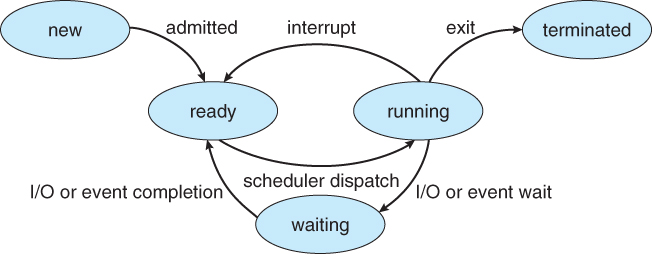
\includegraphics[width=0.45\textwidth]{../figures/figure01}
    \caption{Waiting to Ready CPU Scheduling Scheme [2]}
    \label{fig:fig.waiting-to-ready-cpu-scheduling-scheme-[2]}
\end{figure}

Generally, in order to improve the efficiency of the
CPU, such criteria must be kept to a minimum.~The basic
CPU scheduling scheme is called "waiting to ready" and
illustrated in Figure 1.~In this basic algorithm, if the process
is preemptive, it will not wait any longer to get scheduled.
It will snatch the chance from other lower-priority process.
If the process is having lower priority/non-preemptive, then
it will keep waiting for the resources to release , complete
the event and then get dispatched through the scheduler.
However, a large number of CPU scheduling algorithms that
utilize the aforementioned criteria in their execution were
proposed and analyzed in the literature, for instance:

\begin{itemize}
    \item First Come First Serve~(FCFS): this algorithm executes
    the jobs based on their arrival times, so any process
    that arrives first will be executed.~This algorithm is the
    simplest CPU scheduling algorithm however it produces
    high AWT and ATT.\@
    \item Shortest Job First (SJF): this algorithm executes the jobs
    according to their burst time, so a process with the
    shortest burst time will be executed first.~Hence, this
    algorithm causes starvation of processes that have longer
    burst times.
    \item Round Robin (RR): this algorithm executes jobs with
    specific amounts of time called time quantum.~Therefore,
    all arrival processes will be executed with equal amount
    of time quantum slots.~If a process burst time is greater
    than time quantum it will be blocked and moved to the
    end of the queue and another arrival process will be
    executed.~This algorithm eliminates starvation of processes;
    however, its efficiency depends on selecting the optimal
    value of time quantum.~For example, if the time quantum
    is small, NCS will increase;~however, if the time quantum
    is large, then it will behave as FCFS algorithm [3].
\end{itemize}

\vspace{1em}

There are many researchers developed different solutions
to enhance the performance of RR algorithm, therefore there
is a need to make a comparative study to select the optimal
RR algorithm.~Thus, in this paper, we provide a comparative
study between four different methods that are used to select
optimal time quantum for an RR algorithm that minimizes
the performance criterion factors (i.e., AWT, ATT, ART,
NCS).~The considered RR algorithms include: Adaptive Round
Robin Algorithm [4], Best Time Quantum Round Robin CPU
Scheduling [6], Optimal Round Robin Scheduling Using
Manhattan Distance Algorithm [6], and Improved Round Robin
Scheduling Algorithm [7].~We intentionally chose these four
RR algorithms because their elapsed time are very close to
each other.~Also, we provide extensive simulation results to
evaluate these algorithms according to the aforementioned
factors.\\

The rest of this paper is organized as follows: Section II
presents the related work, Section III describes the Round
Robin Scheduling schemes and its various quantum-based
approaches.~Section IV presents the research methodology and
the simulation results as well as the comparison of the four
algorithms and factors.~Finally, section V concludes the paper